\documentclass[aspectratio=169,11pt]{beamer}

\usepackage{graphicx}
\usepackage{tikz}
\usetikzlibrary{positioning,arrows.meta}
\usepackage{xcolor}
\usepackage{booktabs}
\usepackage{tabularx}
\usepackage{array}
\usepackage{ragged2e}
\usepackage{multirow}
\usepackage{hyperref}

\definecolor{GEUBlue}{RGB}{20,55,105}
\definecolor{GEULightBlue}{RGB}{238,244,251}
\definecolor{GEUGrey}{RGB}{90,90,90}
\definecolor{GEULightGrey}{RGB}{245,246,248}

\usetheme{default}
\setbeamertemplate{navigation symbols}{}
\setbeamertemplate{blocks}[rounded][shadow=false]
\setbeamercolor{normal text}{fg=black,bg=white}
\setbeamercolor{frametitle}{fg=GEUBlue}
\setbeamercolor{structure}{fg=GEUBlue}
\setbeamercolor{block title}{fg=GEUBlue,bg=GEULightBlue}
\setbeamercolor{block body}{fg=black,bg=GEULightBlue}
\setbeamerfont{frametitle}{size=\Large,series=\bfseries}

\newcommand{\GEULogo}{graphicera_logo.png}

% Clean header + Centered Frame Title close to the blue line
\setbeamertemplate{headline}{%
  \begin{tikzpicture}[remember picture,overlay]
    \node[anchor=north east,xshift=-0.30cm,yshift=-0.12cm]
      at (current page.north east)
      {\includegraphics[height=0.62cm]{\GEULogo}};
  \end{tikzpicture}
  \vspace{0.35cm}
}

\setbeamertemplate{frametitle}{%
  \vspace{-0.10cm}
  \centering\insertframetitle\par
  \vspace{0.02cm}
  \textcolor{GEUBlue}{\rule{\textwidth}{0.9pt}}
  \vspace{0.02cm}
}

\setbeamertemplate{footline}{%
  \leavevmode
  \hbox{%
  \begin{beamercolorbox}[wd=.82\paperwidth,ht=0.32cm,dp=0.10cm,leftskip=.3cm]{author in head/foot}
    \tiny Department of Computer Science \& Engineering | Graphic Era (Deemed to be University)
  \end{beamercolorbox}%
  \begin{beamercolorbox}[wd=.18\paperwidth,ht=0.32cm,dp=0.10cm,rightskip=.3cm]{date in head/foot}
    \hfill\tiny\insertframenumber/\inserttotalframenumber
  \end{beamercolorbox}}
}

\newcommand{\smallnote}[1]{\vspace{0.06cm}{\scriptsize\color{GEUGrey}#1}}

\title{\textbf{Project-Based Learning}\\[2mm]\large Phase-II Evaluation}
\author{\textbf{RESQNET: Smart Urban Emergency \&\\Transportation Network Simulator}\\Team ID: DSCPP-III-2026-T070}
\institute{Department of Computer Science \& Engineering\\Graphic Era (Deemed to be University), Dehradun}
\date{Academic Session 2026--27}

\begin{document}

% 1 — TITLE SLIDE
\begin{frame}[plain]
\begin{tikzpicture}[remember picture,overlay]
\draw[GEUBlue,line width=3pt] (current page.north west) -- (current page.north east);
\node[anchor=north east,xshift=-0.45cm,yshift=-0.35cm] at (current page.north east)
{\includegraphics[height=1.0cm]{\GEULogo}};
\node[align=center,text width=.84\paperwidth] at ([yshift=.25cm]current page.center)
{{\color{GEUBlue}\fontsize{26}{30}\selectfont\bfseries PROJECT-BASED LEARNING}\\[3mm]
 {\fontsize{18}{22}\selectfont PHASE-II EVALUATION}\\[7mm]
 {\color{GEUGrey}\Large\bfseries RESQNET: Smart Urban Emergency \&\\Transportation Network Simulator}\\[3mm]
 {\color{GEUBlue}\normalsize Team ID: DSCPP-III-2026-T070}};
\node[align=center,anchor=south,yshift=.42cm] at (current page.south)
{\bfseries Department of Computer Science \& Engineering\\
Graphic Era (Deemed to be University), Dehradun\\[-1mm]
\scriptsize Academic Session 2026--27};
\end{tikzpicture}
\end{frame}

% 2 — TEAM & MENTOR DETAILS
\begin{frame}{Team \& Mentor Details}
\begin{columns}[T,totalwidth=\textwidth]
\column{.48\textwidth}
\begin{block}{Team Information}
\begin{tabular}{@{}ll@{}}
\textbf{Team ID:} & DSCPP-III-2026-T070\\
\textbf{Team Name:} & RESQNET\\
\textbf{Semester:} & 3rd\\
\textbf{Section:} & BTECH\\
\textbf{Domain:} & Graph Algorithms \& DSA
\end{tabular}
\end{block}
\column{.48\textwidth}
\begin{block}{Team Members}
1.\quad Chhavi -- 2510012506\\
2.\quad Tapashya -- 2510011649\\
3.\quad Arpit Chahal -- 2510012000\\[3mm]
\end{block}
\end{columns}
\vspace{2mm}
\begin{block}{Mentor}
Mr. Darshan Singh
\hfill
\textbf{Interactions completed:} 6
\end{block}
\end{frame}

% 3 — PHASE-I RECAP & FEEDBACK INCORPORATED
\begin{frame}{Phase-I Recap \& Feedback Incorporated}
\begin{block}{Phase-I Status}
\small
Finalized the problem statement, identified disaster and vehicle types, modeled the city network as a weighted graph, and planned the priority queue and Dijkstra routing architecture.
\end{block}
\vspace{2mm}
\footnotesize
\begin{columns}[T,totalwidth=\textwidth]
\column{.48\textwidth}
\textbf{\normalsize\color{GEUBlue}Feedback Received}
\begin{itemize}\itemsep2pt
\item Build a role-based login and web interface
\item Expand the fleet to support all specialized rescue vehicles
\item Implement dynamic road closures and shortest-path dispatch
\end{itemize}
\column{.48\textwidth}
\textbf{\normalsize\color{GEUBlue}Changes Incorporated}
\begin{itemize}\itemsep2pt
\item Built user and dispatcher portals with interactive 10-junction map
\item Configured 80 response vehicles across 25 emergency categories
\item Implemented Dijkstra routing, road-closure toggles, and ETA engine
\end{itemize}
\end{columns}
\end{frame}

% 4 — PROBLEM STATEMENT & FINALIZED OBJECTIVES
\begin{frame}{Problem Statement \& Finalized Objectives}
\begin{block}{Problem Statement}
\small
Design a multi-disaster city simulation that prioritizes concurrent emergencies, dispatches optimal response vehicles, and dynamically reroutes around road closures using Data Structures.
\end{block}
\vspace{1.5mm}
\footnotesize
\textbf{\normalsize\color{GEUBlue}Finalized Objectives}
\begin{enumerate}\itemsep1.5pt
\item \textbf{Incident Triage:} Support 25 emergency types and rank pending reports by priority score ($10 \times \text{severity} + 0.5 \times \text{people}$).
\item \textbf{Weighted City Graph:} Model 10 junctions and 14 roads with Dijkstra shortest-path routing and road-closure bypass.
\item \textbf{Multi-Vehicle Allocation:} Match required unit types from an 80-vehicle fleet based on fastest travel time (ETA).
\item \textbf{Interactive Portal:} Provide role-based Citizen Reporting and Dispatcher Control views synced with the core engine.
\end{enumerate}
\end{frame}

% 5 — UPDATED SYSTEM ARCHITECTURE / WORKFLOW
\begin{frame}{Updated System Architecture / Workflow}
\begin{center}
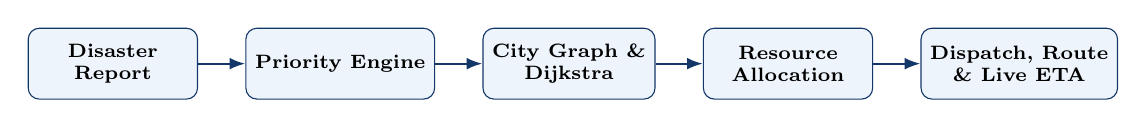
\begin{tikzpicture}[
node distance=6mm,
box/.style={rectangle,rounded corners,draw=GEUBlue,fill=GEULightBlue,
minimum width=2.15cm,minimum height=9mm,align=center,font=\scriptsize\bfseries},
arrow/.style={-{Latex[length=2mm]},thick,draw=GEUBlue}
]
\node[box] (a) {Disaster\\Report};
\node[box,right=of a] (b) {Priority Engine};
\node[box,right=of b] (c) {City Graph \&\\Dijkstra};
\node[box,right=of c] (d) {Resource\\Allocation};
\node[box,right=of d] (e) {Dispatch, Route\\\& Live ETA};
\draw[arrow] (a)--(b); \draw[arrow] (b)--(c); \draw[arrow] (c)--(d); \draw[arrow] (d)--(e);
\end{tikzpicture}
\end{center}
\vspace{3mm}
\footnotesize
\begin{columns}[T,totalwidth=\textwidth]
\column{.48\textwidth}
\textbf{\normalsize\color{GEUBlue}Major Components}
\begin{itemize}\itemsep2pt
\item \textbf{Priority \& Store:} Incident queue, severity scoring, user auth
\item \textbf{Graph \& Fleet:} 10-junction city graph, 80-vehicle fleet pool
\item \textbf{Web Portal:} Citizen reporting \& Dispatcher control room
\end{itemize}
\column{.48\textwidth}
\textbf{\normalsize\color{GEUBlue}Changes Since Phase-I}
\begin{itemize}\itemsep2pt
\item Expanded from 7 planned disasters to 25 emergency categories
\item Added direct air-routing ($16.7\text{ m/s}$) for Helicopter units
\item Added interactive map with live status \& route confirmation
\end{itemize}
\end{columns}
\end{frame}

% 6 — MODULE DESIGN: PHASE 1 - INCIDENT & RESOURCE MODULE
\begin{frame}{Module Design: Phase 1 -- Incident \& Resource Module}
\footnotesize
\begin{columns}[T,totalwidth=\textwidth]
\column{.48\textwidth}
\textbf{\normalsize\color{GEUBlue}Phase 1 Modules}
\begin{enumerate}\itemsep2pt
\item \textbf{\texttt{common.h}:} Shared constants, 25 incident \& 8 vehicle enums
\item \textbf{\texttt{incident.h/c}:} Incident store, priority score, pending lookup
\item \textbf{\texttt{types.h/c}:} Vehicle requirements \& safety precautions
\item \textbf{\texttt{fleet.h/c}:} 80-unit fleet loader from \texttt{data/vehicles.txt}
\item \textbf{\texttt{auth.h/c} \& \texttt{io.h/c}:} Role authentication \& input validation
\end{enumerate}
\column{.48\textwidth}
\textbf{\normalsize\color{GEUBlue}Functional Requirements}
\begin{itemize}\itemsep2pt
\item Record emergency type, junction (1--10), severity, and people count
\item Calculate priority score $\text{Score} = 10.0 \times \text{severity} + 0.5 \times \text{people}$
\item Provide instant incident-specific safety precautions to reporters
\item Track incident lifecycle (\texttt{REPORTED}, \texttt{DISPATCHED}, \texttt{RESOLVED})
\end{itemize}
\end{columns}
\end{frame}

% 7 — MODULE DESIGN: PHASE 2 - GRAPH ROUTING & DISPATCH
\begin{frame}{Module Design: Phase 2 -- Graph Routing \& Dispatch}
\footnotesize
\begin{columns}[T,totalwidth=\textwidth]
\column{.48\textwidth}
\textbf{\normalsize\color{GEUBlue}Phase 2 Modules}
\begin{enumerate}\itemsep2pt
\item \textbf{\texttt{city.h/c}:} Weighted graph, Dijkstra algorithm, road closures
\item \textbf{\texttt{dispatch.h/c}:} \texttt{vehicle\_eta()}, \texttt{find\_best()}, \texttt{dispatch\_incident()}
\item \textbf{\texttt{main.c}:} User \& Dispatcher workflows and engine integration
\item \textbf{Web Portal:} React 19 Citizen \& Dispatcher control interfaces
\end{enumerate}
\column{.48\textwidth}
\textbf{\normalsize\color{GEUBlue}Functional Requirements}
\begin{itemize}\itemsep2pt
\item Compute shortest travel time (seconds) across 14 bidirectional roads
\item Bypass \texttt{BLOCKED} roads dynamically and recompute alternate paths
\item Route Helicopters via straight-line distance ignoring road blocks
\item Lock assigned vehicles until the dispatcher resolves the incident
\end{itemize}
\end{columns}
\end{frame}

% 8 — CODE PIPELINE: PHASE 1 & PHASE 2
\begin{frame}{Code Pipeline -- Phase 1 \& Phase 2}
\footnotesize
\begin{block}{Phase 1 -- Incident Reporting \& Priority Pipeline}
\centering
\texttt{user\_report()} $\longrightarrow$ \texttt{store\_add()} $\longrightarrow$ \texttt{priority\_score()} $\longrightarrow$ \texttt{precaution\_for()} $\longrightarrow$ \texttt{store\_save()} $\longrightarrow$ \texttt{data/incidents.txt} (\texttt{REPORTED})
\end{block}

\vspace{3mm}

\begin{block}{Phase 2 -- Dijkstra Routing \& Fleet Dispatch Pipeline}
\centering
\texttt{store\_best\_pending()} $\longrightarrow$ \texttt{needs\_for()} $\longrightarrow$ \texttt{find\_best()} $\longrightarrow$ \texttt{city\_shortest\_path()} / \texttt{heli\_seconds()} $\longrightarrow$ \texttt{dispatch\_incident()} $\longrightarrow$ \texttt{DISPATCHED}
\end{block}

\vspace{2mm}
\smallnote{Each incident is assigned up to 4 nearest available units; marking an incident \texttt{RESOLVED} releases its vehicles back to the available pool.}
\end{frame}

% 9 — TECHNOLOGY STACK & DEVELOPMENT METHODOLOGY
\begin{frame}{Technology Stack \& Development Methodology}
\footnotesize
\begin{columns}[T,totalwidth=\textwidth]
\column{.48\textwidth}
\begin{block}{Technology Stack}
\begin{itemize}\itemsep2pt
\item \textbf{Core Engine:} C / C++ (\texttt{gcc -O2 -Wall -Wextra})
\item \textbf{Data Structures:} Weighted Graph, Priority Queue, Structs
\item \textbf{Algorithms:} Dijkstra Shortest Path, Euclidean Air-Routing
\item \textbf{Web Portal:} React 19, TypeScript, Vite, Tailwind CSS, Supabase
\item \textbf{Version Control:} Git / GitHub
\end{itemize}
\end{block}
\column{.48\textwidth}
\begin{block}{Development Methodology}
\begin{enumerate}\itemsep2pt
\item Requirement Analysis \& Graph Modeling
\item Modular Header \& Struct Design
\item Priority Queue \& Fleet Loader Implementation
\item Dijkstra Routing \& Dispatcher Integration
\item Scenario Testing \& Web Portal Verification
\end{enumerate}
\end{block}
\end{columns}
\end{frame}

% 10 — IMPLEMENTATION OF PBL COURSE CONCEPTS
\begin{frame}{Implementation of PBL Course Concepts}
\footnotesize
\begin{center}
\renewcommand{\arraystretch}{1.35}
\begin{tabularx}{.96\textwidth}{@{}>{\bfseries}p{3.2cm}X p{4.2cm}@{}}
\toprule
Course & Concepts Actually Implemented & Project Module\\
\midrule
Data Structures & Weighted Graph, Priority Selection, Dynamic Arrays, Lookup Tables & \texttt{city.h/c}, \texttt{incident.h/c}, \texttt{fleet.h/c}, \texttt{types.h/c}\\
Modular Design & Structured ADTs, Encapsulation, Header Guards, Enum State Machines & \texttt{common.h}, \texttt{dispatch.h/c}, \texttt{auth.h/c}, \texttt{io.h/c}\\
\midrule
Algorithms & Dijkstra Shortest Path, Greedy Unit Selection, Euclidean Air ETA & \texttt{city\_shortest\_path()}, \texttt{find\_best()}, \texttt{vehicle\_eta()}\\
File Handling & Persistent Incident Store, Fleet Config, City Graph \& User Records & \texttt{city.txt}, \texttt{vehicles.txt}, \texttt{incidents.txt}, \texttt{users.txt}\\
\bottomrule
\end{tabularx}
\end{center}
\end{frame}

% 11 — DEVELOPMENT & IMPLEMENTATION PROGRESS
\begin{frame}{Development \& Implementation Progress}
\footnotesize
\begin{center}
\renewcommand{\arraystretch}{1.35}
\begin{tabularx}{.96\textwidth}{@{}p{3.8cm}p{2.0cm}X@{}}
\toprule
\textbf{Module} & \textbf{Status} & \textbf{Work Completed}\\
\midrule
Phase 1 -- City Graph \& Fleet Pool & \textbf{\color{green!50!black}Completed} & \texttt{city.h/c} (10 junctions, 14 roads), \texttt{fleet.h/c} (80 response units)\\
Phase 1 -- Incident \& Priority Engine & \textbf{\color{green!50!black}Completed} & \texttt{incident.h/c}, \texttt{types.h/c} (25 emergency types \& precautions)\\
Phase 2 -- Dijkstra \& Fleet Dispatch & \textbf{\color{green!50!black}Completed} & \texttt{dispatch.h/c} (shortest-path ETA, air routing, road closures)\\
Phase 2 -- Role-Based Web Portal & \textbf{\color{green!50!black}Completed} & Citizen reporting \& Dispatcher control views with live status sync\\
Phase 3 -- Resilience \& Multi-City & \textbf{\color{orange!80!black}Pending} & Articulation-point resilience analysis and hospital bed capacity\\
\bottomrule
\end{tabularx}
\end{center}
\end{frame}

% 12 — WORKING PROTOTYPE: PHASE 1 -- USER REPORTING & STATUS
\begin{frame}[fragile]{Working Prototype: Phase 1 -- User Reporting}
\footnotesize
\begin{columns}[T,totalwidth=\textwidth]
\column{.45\textwidth}
\textbf{\normalsize\color{GEUBlue}Implemented Features}
\begin{itemize}\itemsep2pt
\item \textbf{Live Web Portal:} \href{https://spline-stall-88999147.figma.site}{\texttt{spline-stall-88999147.figma.site}}
\item \textbf{Role Authentication:} Separate Citizen (\texttt{U}) and Dispatcher (\texttt{D}) login
\item \textbf{25 Emergency Types:} Quick-pick situations \& junction selector
\item \textbf{Live Precautions:} Shows assigned units, routes, ETAs \& safety steps
\end{itemize}
\column{.52\textwidth}
\begin{block}{Phase 1 CLI Output (\texttt{./resqnet})}
\tiny
\begin{verbatim}
Welcome taps (User)
--- Your current reports ---
------------------------------------------------------------
 #1: Fire Emergency at Main Road
 Status: DISPATCHED
 Your note: Vehicle on fire or smoke
  [GO] FireTruck-F2 (Fire Truck) from Base Station
       Route   : Base Station -> Main Road
       ETA     : 60 s (about 1 min)
  [GO] Ambulance-A3 (Ambulance) from City Hospital
       Route   : City Hospital -> Station Chowk -> Main Road
       ETA     : 90 s (about 2 min)
 Precautions until the team arrives:
   Leave the area and keep others away. Do not use lifts.
\end{verbatim}
\end{block}
\end{columns}
\end{frame}

% 13 — WORKING PROTOTYPE: PHASE 2 -- DISPATCHER & DIJKSTRA ROUTING
\begin{frame}[fragile]{Working Prototype: Phase 2 -- Dispatcher Engine}
\footnotesize
\begin{columns}[T,totalwidth=\textwidth]
\column{.45\textwidth}
\textbf{\normalsize\color{GEUBlue}Implemented Features}
\begin{itemize}\itemsep2pt
\item \textbf{Priority Ordering:} Scores incidents ($92.0$ vs $81.5$) for next dispatch
\item \textbf{Dijkstra Shortest Path:} Computes junction-by-junction route \& ETA
\item \textbf{Multi-Unit Match:} Dispatches Fire Truck, Ambulance, and Police
\item \textbf{Road Status Control:} Toggles any of the 14 city roads \texttt{open}/\texttt{BLOCKED}
\end{itemize}
\column{.52\textwidth}
\begin{block}{Phase 2 CLI Output (\texttt{./resqnet})}
\tiny
\begin{verbatim}
Welcome Chhavi (Dispatcher)
------------------------------------------------------------
 #2: Gas Explosion at Park Lane  [DISPATCHED]
 Severity 9/10 | People 4 | Priority 92.0 | Reported by taps
  [GO] FireTruck-F1 (Fire Truck) from Base Station
       Route   : Base Station -> Park Lane
       ETA     : 50 s (about 1 min)
  [GO] Ambulance-A1 (Ambulance) from City Hospital
       Route   : City Hospital -> Civil Lines -> Bus Stand
                 -> Market Square -> Park Lane
       ETA     : 180 s (about 3 min)
  [GO] Police-P5 (Police) from Park Lane | ETA: 0 s
------------------------------------------------------------
\end{verbatim}
\end{block}
\end{columns}
\end{frame}

% 14 — TESTING, RESULTS & VALIDATION
\begin{frame}{Testing, Results \& Validation}
\footnotesize
\begin{center}
\renewcommand{\arraystretch}{1.35}
\begin{tabularx}{.96\textwidth}{@{}p{2.8cm}X X p{1.2cm}@{}}
\toprule
Module & Expected Result & Observed Result & Status\\
\midrule
\texttt{city.c} (Dijkstra) & Compute fastest path \& bypass closed roads & Optimal path \& alternate reroute verified & \textbf{\color{green!50!black}Pass}\\
\texttt{incident.c} (Priority) & Select highest score ($10S + 0.5P$) first & Priority 92.0 selected before 81.5 & \textbf{\color{green!50!black}Pass}\\
\texttt{fleet.c} \& \texttt{types.c} & Load fleet \& map required vehicle types & 80 vehicles loaded; exact needs matched & \textbf{\color{green!50!black}Pass}\\
\texttt{dispatch.c} & Assign nearest free units \& calculate ETA & Closest available units assigned with ETA & \textbf{\color{green!50!black}Pass}\\
\texttt{auth.c} \& Web UI & Enforce role access \& sync dispatch status & User \& Dispatcher views synced accurately & \textbf{\color{green!50!black}Pass}\\
\bottomrule
\end{tabularx}
\end{center}
\end{frame}

% 15 — GITHUB REPOSITORY & DEVELOPMENT ACTIVITY
\begin{frame}{GitHub Repository \& Development Activity}
\footnotesize
\begin{columns}[T,totalwidth=\textwidth]
\column{.48\textwidth}
\textbf{\normalsize\color{GEUBlue}Repository Information}
\begin{itemize}\itemsep2.5pt
\item \textbf{GitHub:} \href{https://github.com/mchhavi929-ship-it/Resqnet}{\texttt{mchhavi929-ship-it/Resqnet}}
\item \textbf{Live Demo:} \href{https://spline-stall-88999147.figma.site}{\texttt{spline-stall-88999147.figma.site}}
\item \textbf{README.md:} Updated with architecture \& setup guide
\item \textbf{Contributors:} Chhavi, Tapashya, Arpit Chahal
\item \textbf{Branch:} \texttt{main}
\end{itemize}
\column{.48\textwidth}
\textbf{\normalsize\color{GEUBlue}Development Activity}
\begin{itemize}\itemsep2.5pt
\item Structured into \texttt{include/}, \texttt{src/}, \texttt{data/}, and \texttt{frontend/}
\item Modular commits across graph, fleet, priority, and UI
\item Verified end-to-end reporting and dispatch workflows
\item Individual module ownership tracked in repository
\item Complete documentation and datasets included
\end{itemize}
\end{columns}
\end{frame}

% 16 — INDIVIDUAL CONTRIBUTION
\begin{frame}{Individual Contribution}
\footnotesize
\begin{center}
\renewcommand{\arraystretch}{1.45}
\begin{tabularx}{.96\textwidth}{@{}>{\RaggedRight\arraybackslash}p{3.4cm}>{\RaggedRight\arraybackslash}p{2.0cm}>{\RaggedRight\arraybackslash}X@{}}
\toprule
\textbf{Member} & \textbf{Role} & \textbf{Technical Contribution} \\
\midrule
Chhavi -- 2510012506 & Team Lead & Built \texttt{city.h/c} (graph, Dijkstra, road closures), \texttt{dispatch.h/c} (ETA \& route display), \texttt{common.h}, and integrated \texttt{main.c} \& Web UI.\\
Tapashya -- 2510011649 & Developer & Built \texttt{fleet.h/c} (vehicle structs \& fleet loader), \texttt{types.h/c} (incident vehicle needs), and coordinated \texttt{find\_best()} \& \texttt{dispatch\_incident()}.\\
Arpit Chahal -- 2510012000 & Developer & Built \texttt{incident.h/c} (incident store, priority score, pending selection), \texttt{io.h/c} (input helpers), and \texttt{auth.h/c} with \texttt{data/*.txt}.\\
\bottomrule
\end{tabularx}
\end{center}
\end{frame}

% 17 — CHALLENGES, ROADMAP & REFERENCES
\begin{frame}{Challenges, Phase-III Roadmap \& References}
\footnotesize
\begin{columns}[T,totalwidth=\textwidth]
\column{.48\textwidth}
\textbf{\normalsize\color{GEUBlue}Challenges \& Solutions}
\begin{itemize}\itemsep1.5pt
\item \textbf{Blocked Road Rerouting:} Handled unreachable paths cleanly and switched to alternate Dijkstra routes
\item \textbf{Busy Fleet Tracking:} Prevented double-booking by scanning active \texttt{DISPATCHED} incidents before allocation
\end{itemize}
\vspace{1.5mm}
\textbf{\normalsize\color{GEUBlue}Phase-III Roadmap}
\begin{enumerate}\itemsep1.5pt
\item Articulation-point detection for critical city junctions
\item Hospital capability and bed-capacity matching
\item Multi-scenario stress testing and final evaluation demo
\end{enumerate}

\column{.48\textwidth}
\textbf{\normalsize\color{GEUBlue}References}
\begin{enumerate}\itemsep1.5pt
\item Cormen et al., \textit{Introduction to Algorithms}
\item E.\ Balagurusamy, \textit{Object Oriented Programming with C++}, 8th Ed.
\item Herbert Schildt, \textit{The Complete Reference C++}, 4th Ed.
\item \texttt{cppreference.com} \& React Documentation
\end{enumerate}
\vspace{3mm}
\begin{center}
\colorbox{GEUBlue}{\parbox{.78\textwidth}{\centering\color{white}\textbf{Thank You}\\Questions \& Suggestions}}
\end{center}
\end{columns}
\end{frame}

\end{document}